\subsubsection{Descrizione generale}
Questo servizio ha l'importante compito di far partire automaticamente,
ogni intervallo di tempo predefinito, l'esecuzione del gruppo di servizi \textbf{S4}.
La funzione di timer, che andrà a notificare la funzione Lambda responsabile vera e propria dello
scheduling, è affidata ad una regola di Amazon EventBridge.

\subsubsection{Diagramma delle classi}
\begin{figure}[H]
    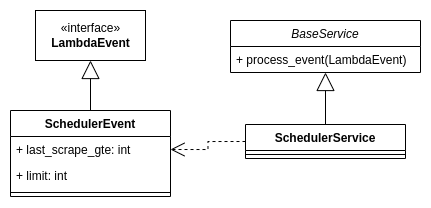
\includegraphics[width=8cm]{sezioni/images/cd_scheduler.png}
    \centering
    \caption{Scheduler Service - Diagramma delle classi}
\end{figure}

\subsubsection{Diagramma di sequenza}
\begin{figure}[H]
    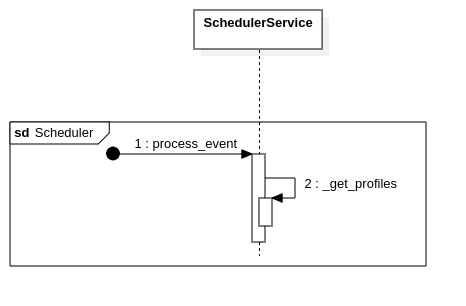
\includegraphics[width=8cm]{sezioni/images/sd_scheduler.png}
    \centering
    \caption{Scheduler Service - Diagramma di sequenza}
\end{figure}

\subsubsection{Schemi I/O}
\paragraph*{Input} esempio di evento in input, in formato JSON\G{}.
\begin{lstlisting}[language=JSON]
{
    "last_scrape_gte": 12,
    "limit": 10
}
\end{lstlisting}
Descrizione:
\begin{itemize}
    \item \verb|last_scrape_gte|: minimo intervallo di tempo passato dall'ultima azione di scraping
    per considerare un profilo social (misurato in ore);
    \item \verb|limit|: numero massimo di profili social da trattare. 
\end{itemize}

\paragraph*{Output} esempio di risposta in output, in formato JSON\G{}.
\begin{lstlisting}[language=JSON]
{
    "profiles_count": 2,
    "profiles": [
        {
            "id": 1,
            "username": "testuser1"
        },
        {
            "id": 2,
            "username": "testuser2"
        }
    ],
}
\end{lstlisting}
Descrizione:
\begin{itemize}
    \item \verb|profiles_count|: numero di profili social trattati;
    \item \verb|profiles|: array di profili social. 
\end{itemize}

\subsubsection{Intervallo temporale}
L'intervallo temporale scelto, sulla base del quale poi eseguire ad intervalli regolari lo scheduling,
è stato impostato a 30 minuti.

\subsubsection{Regole di scheduling}
La scelta di quali profili social sottoporre ad una esecuzione di \textbf{S4}, avviene sulla base del
campo \verb|SocialProfile.last_scraped|, memorizzato nel database. Verranno quindi scelti per l'esecuzione
i profili social dove la differenza fra data e ora attuali e \verb|last_scraped| è di 12 ore.
